%% inequality.tex
%%
%% Intro to inequality metrics for the``Communities'' course of the
%%   Official Master on Libre Software (URJC)
%%   http://master.libresoft.es

%%---------------------------------------------------------------------
%%---------------------------------------------------------------------
\section{Analysis of inequality}

%%---------------------------------------------------------------

\begin{frame}
\frametitle{Inequality}

The aim of this analysis is to measure the inequality level in the distribution of a certain
paramenter among the members of a population. It is frequently associated with economics,
well-fare studies.\\

\begin{center}
 \begin{quotation}
  \textit{For example: distribution of wealth or income among inhabitants of a country.}
  \end{quotation}
\end{center}

\end{frame}

%%---------------------------------------------------------------

\begin{frame}
\frametitle{How to study inequalities}

\begin{itemize}
  \item Graphical methods: Lorenz curve
  \item Numerical methods: Inequality coefficients
  \begin{itemize}
   \item Gini.
   \item Atkinson.
   \item Ricci-Schutz.
   \item Theil.
   \item Kolm.
  \end{itemize}

\end{itemize}

\end{frame}

%%---------------------------------------------------------------

\begin{frame}
\frametitle{Example}

\textbf{Number of commits per developer}
\begin{itemize}
\item Consider the following distribution of commits performed by each developer over
the whole history of a FLOSS project:
\end{itemize}

\textbf{Case A}
\begin{tabular}{|c|c|c|c|c|c|c|c|}
\hline
\textbf{Nick} & Dev1 & Dev2 & Dev3 & Dev4 & Dev5 & Dev6 & Dev7 \\
\hline
\textbf{Ncommits} & 1 & 1 & 1& 2 & 5 & 50 & 310 \\
\hline
\end{tabular}

\vspace{1cm}

\textbf{Case B}
\begin{tabular}{|c|c|c|c|c|c|c|c|}
\hline
\textbf{Nick} & Dev1 & Dev2 & Dev3 & Dev4 & Dev5 & Dev6 & Dev7 \\
\hline
\textbf{Ncommits} & 1 & 2 & 10& 20 & 50 & 70 & 120 \\
\hline
\end{tabular}

\end{frame}

%%---------------------------------------------------------------

\begin{frame}
\frametitle{Example}

\begin{itemize}
  \item Possible questions:
  \begin{itemize}
   \item Is it possible to make a graphical representation, suitable for
analyzing the inequality in the distribution of commits among developers?

   \item Can we compute a numerical coefficient to summarize this inequality
information?
  \end{itemize}

\end{itemize}

\end{frame}

%%---------------------------------------------------------------------
\subsection{The Lorenz curve}

%%---------------------------------------------------------------

\begin{frame}
\frametitle{The aim of the Lorenz curve}

\begin{itemize}
  \item Graphical representation of the distribution of a certain parameter among
population members.
\end{itemize}

\begin{figure}
 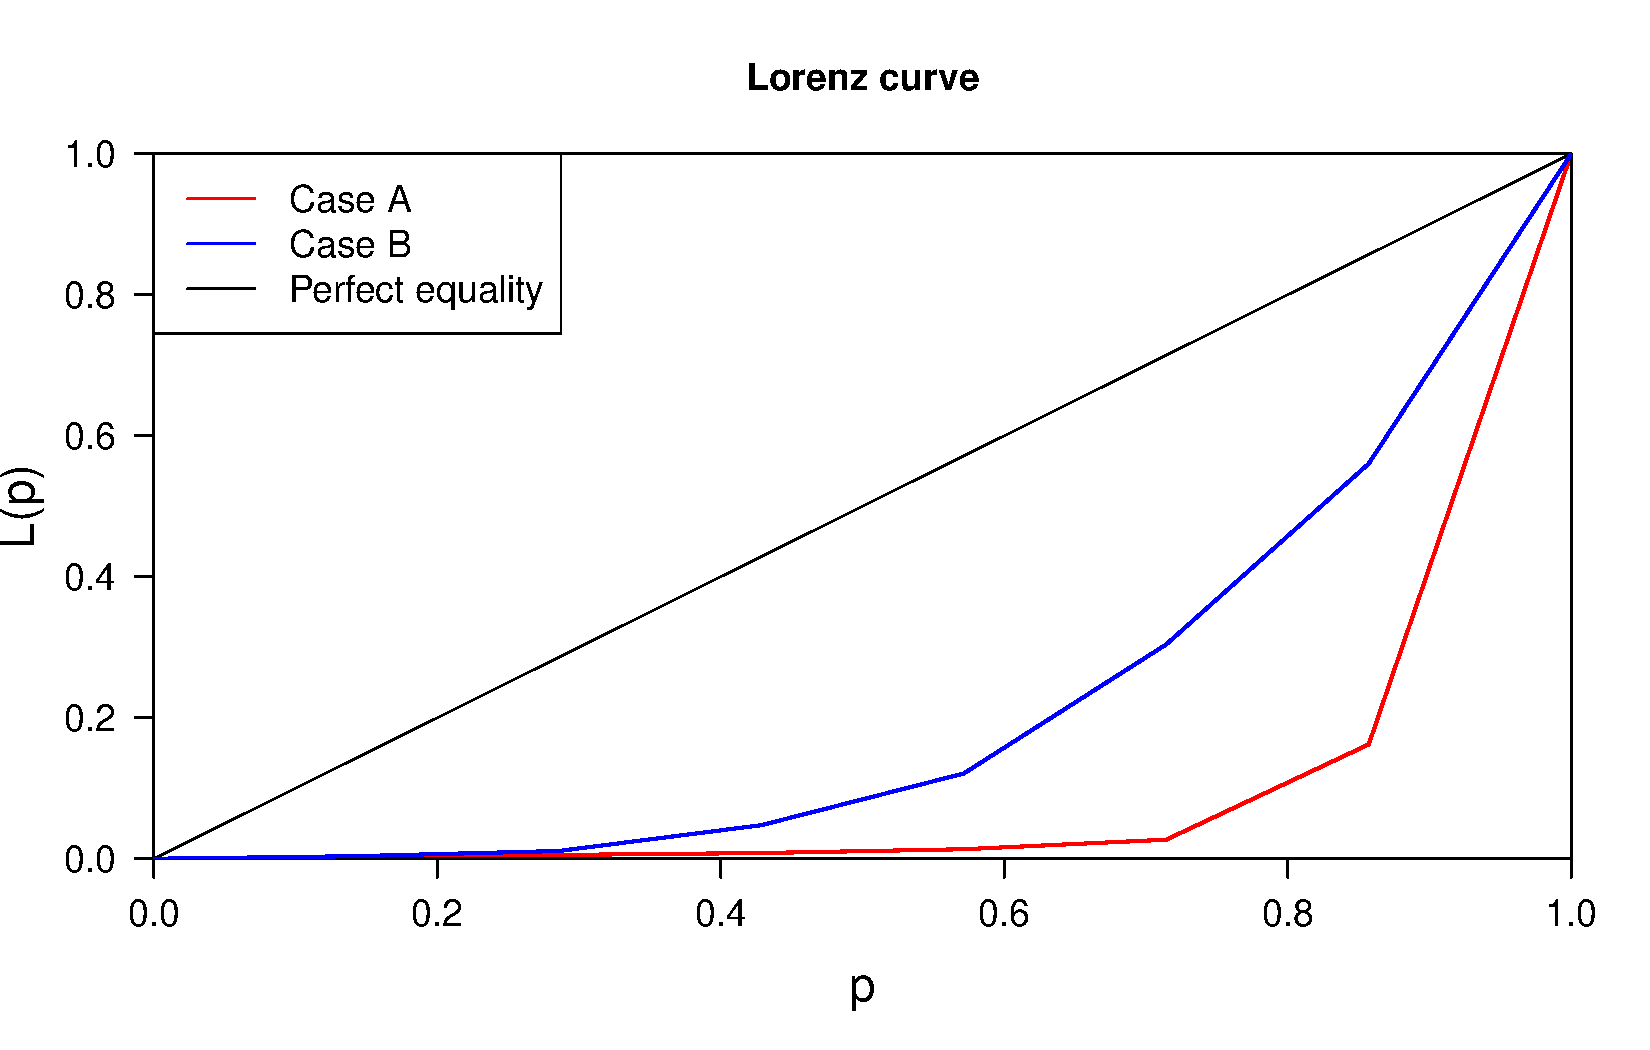
\includegraphics[height=6.5cm]{figs/example-Lorenz}
\end{figure}

\end{frame}

%%---------------------------------------------------------------

\begin{frame}
\frametitle{Lorenz curve step-by-step}

\begin{enumerate}
 \item Order the values in ascending rank.
 \item Calculate cumulative values of measured parameter $u_i$.
 \item Calculate percentage values (proportions) for X ($p_i$) and Y ($L(p_i)$) variables.
 \item Plot the graph along with the line of perfect equality.
\end{enumerate}

\end{frame}

%%---------------------------------------------------------------

\begin{frame}
\frametitle{Lorenz curve step-by-step}

\begin{itemize}
 \item Let $n_i$ be the index of each individual member.
 \item Let $N$ be the size of the population.
 \item Let $x_i$ be the value assigned to each member of this population.
\end{itemize}

\begin{equation}
 u_i=\sum_{j=1}^{j=i}[x_j]
\end{equation}

\begin{equation}
 p_i=\frac{n_i}{N} (\%)
\end{equation}

\begin{equation}
 L(p_i)=\frac{u_i}{u_N} (\%)
\end{equation}


\end{frame}

%%---------------------------------------------------------------

\begin{frame}
\frametitle{Example}

\textbf{Number of commits per developer}
\begin{itemize}
\item Consider the following distribution of commits performed by each developer over
the whole history of a FLOSS project:
\end{itemize}

\textbf{Case A}
\begin{tabular}{|c|c|c|c|c|c|c|c|}
\hline
\textbf{Nick} & Dev1 & Dev2 & Dev3 & Dev4 & Dev5 & Dev6 & Dev7 \\
\hline
$n_i$ & 1 & 2 & 3 & 4 & 5 & 6 & 7 \\
\hline 
\textbf{Ncommits} ($x_i$) & 1 & 1 & 1& 2 & 5 & 50 & 310 \\
\hline
\textbf{$u_i$} & 1 & 2 & 3 & 5 & 10 & 60 & 370 \\
\hline
\textbf{$p_i$ (\%)} & 14.3 & 28.5 & 42.9 & 57.1 & 71.4 & 85.8 & 100 \\
\hline
\textbf{$L(p_i)$ (\%)} & 0.27 & 0.54 & 0.81 & 1.35 & 2.70 & 16.22 & 100 \\
\hline
\end{tabular}

\end{frame}

%%---------------------------------------------------------------

\begin{frame}
\frametitle{Example}

\begin{itemize}
  \item And finally, we plot $L(p_i)$ (Y-axis) vs. $p_i$ (X-axis).
\end{itemize}

\begin{figure}
 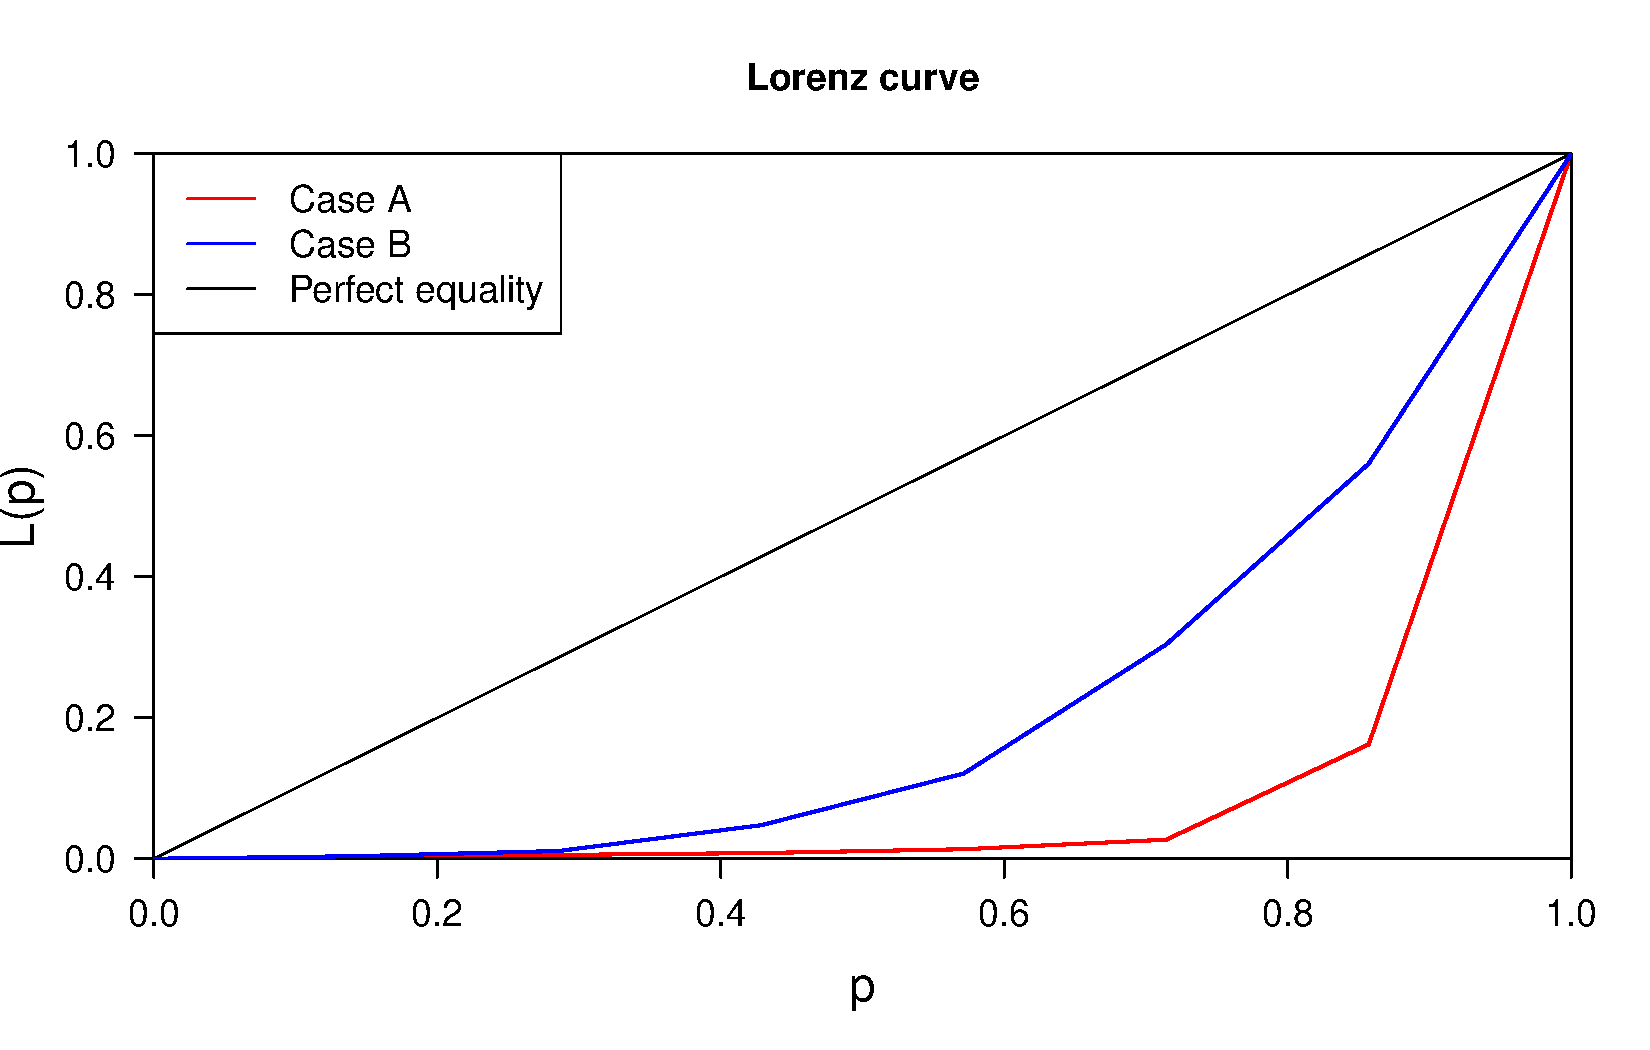
\includegraphics[height=6.5cm]{figs/example-Lorenz}
\end{figure}

\end{frame}

%%---------------------------------------------------------------

\begin{frame} [fragile]
\frametitle{How to do it with R}

\begin{itemize}
  \item We need the \texttt{ineq} library.
\end{itemize}

\begin{footnotesize}
\begin{verbatim}
> library(ineq)
> a = c(1,1,1,2,5,50,310)
> b = c(1,2,10,20,50,70,120)
> Lc.a = Lc(a)
> Lc.b = Lc(b)
>
> pdf("example-Lorenz.pdf", width = 11, height=7, 
+ pointsize = 15)
> plot(Lc.a, col="red")
> plot(Lc.b, col="blue")
> legend("topleft", c("Case A", "Case B", "Perfect equality"), 
+ col = c("red", "blue", "black"), lty = 1)
> dev.off()
\end{verbatim}
\end{footnotesize}

\end{frame}

%%---------------------------------------------------------------

\begin{frame}
\frametitle{Lorenz curve: conclusions}

\begin{itemize}
 \item Graphical representation of concentration of a certain distribution.
 \item Very useful offer a general picture of the whole case study.
 \item It is invariant with respect to scale changes.
 \item It is difficult to compare different Lorenz curves (specially if they cross).
 \item We need a summarizing coefficient to compare different distributions of
inequality.
 \item Solution:Inequality coefficients.
\end{itemize}

\end{frame}

%%---------------------------------------------------------------------
\subsection{The Gini Coefficient}

%%---------------------------------------------------------------------

%%---------------------------------------------------------------

\begin{frame}
\frametitle{Aim of the Gini coefficient}

\begin{itemize}
 \item Summary value to represent inequality of a distribution.
 \item Useful when we need to compare inequalities in different populations.
 \item But we loose more information about the precise details of the distribution.
 \item It can also be a bad approximation if the size of the population
is not large enough (rule of thumb:  $N\geq30$).
\end{itemize}

\end{frame}

%%---------------------------------------------------------------

\begin{frame} [fragile]
\frametitle{Expression and range for Gini coeff.}

\begin{itemize}
 \item Calculating the Gini coefficient (from values for the Lorenz curve).
 \item Values between 0 and 1. 0 means perfect equality, 1 for extreme inequality.
\end{itemize}

\begin{equation}
   G=\frac{\displaystyle\sum_{i=1}^{n-1}[p_i-L(p_i)]}{\displaystyle\sum_{i=1}^{n-1} p_i}; \;\;\;\; G \in [0,1]
%    \label{eq:gini-coeff}
\end{equation}

\end{frame}

%%---------------------------------------------------------------

\begin{frame}
\frametitle{Graphical interpretation Gini coeff.}

\begin{figure}
 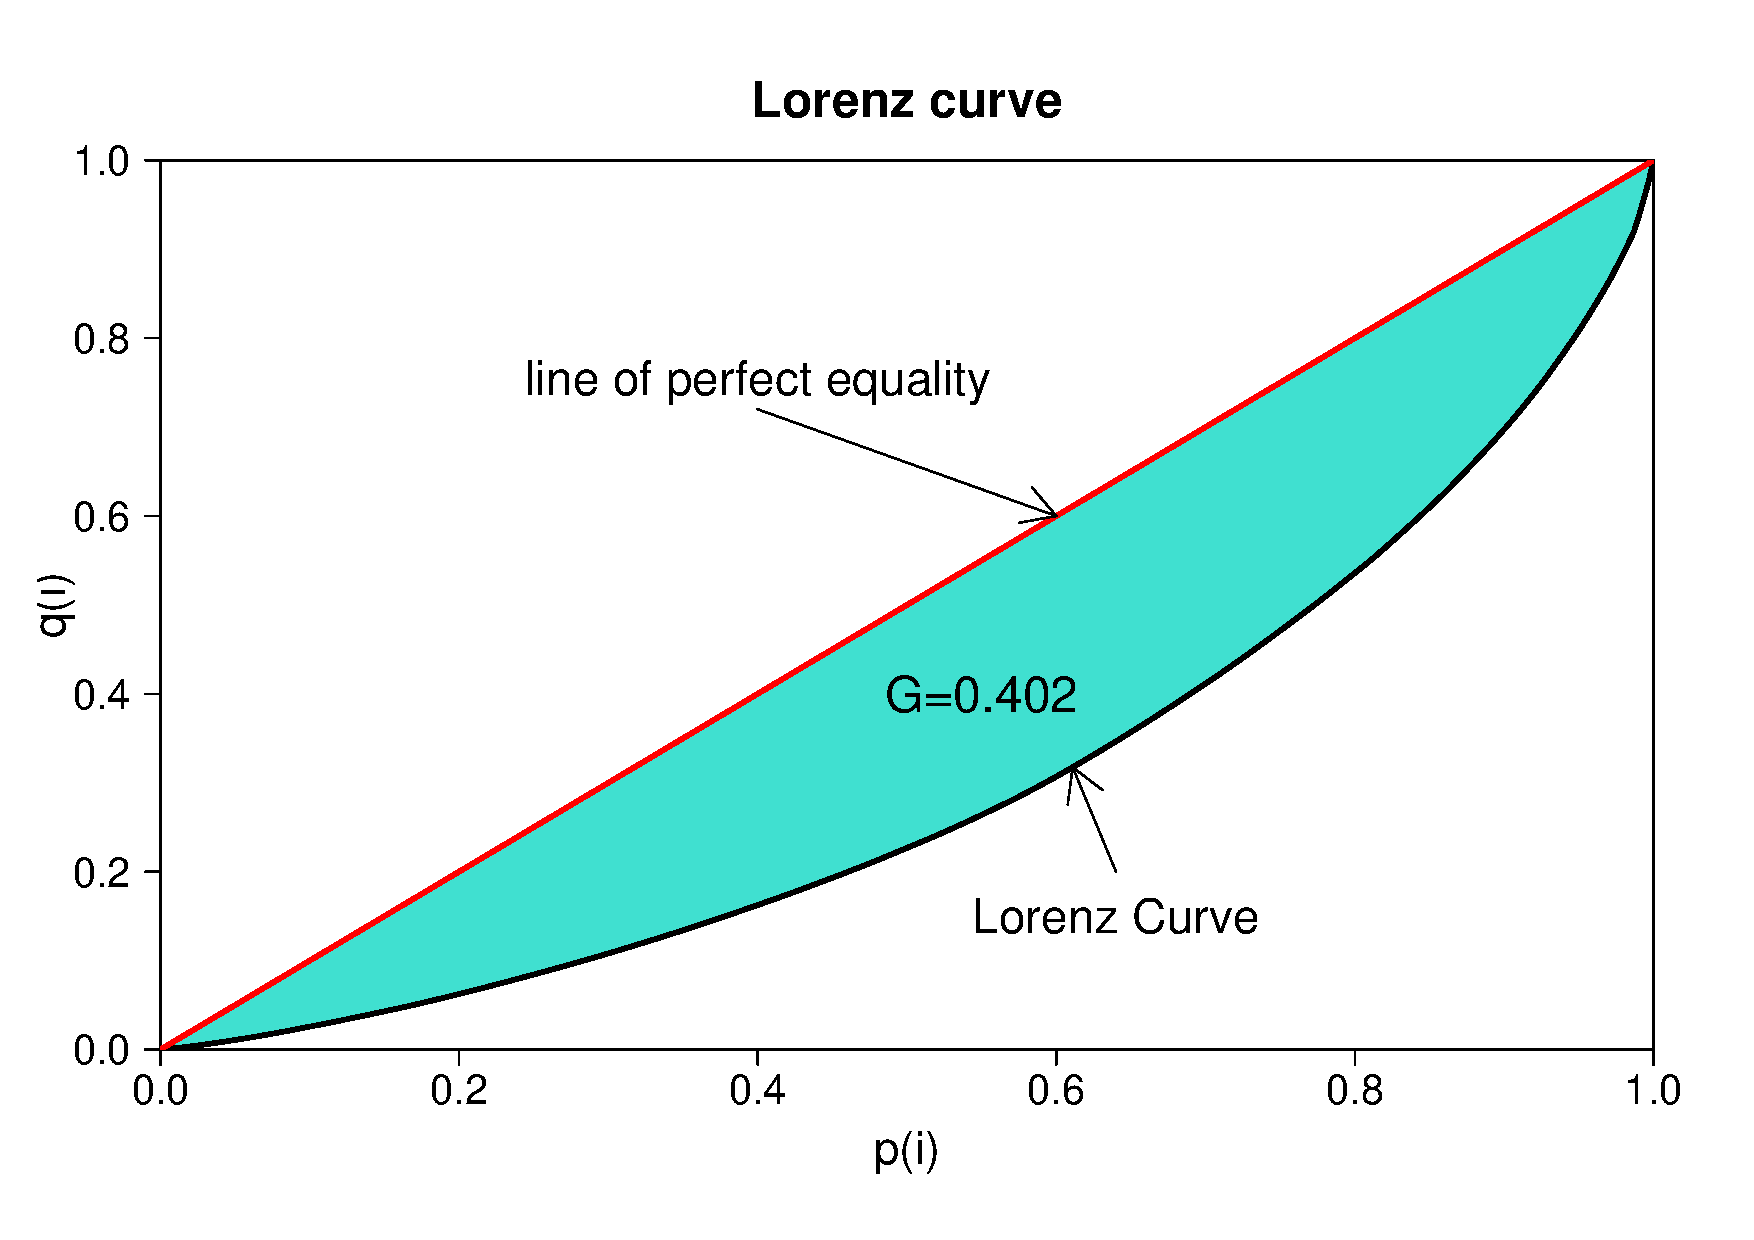
\includegraphics[height=6.5cm]{figs/example-gini}
\end{figure}

\end{frame}

%%---------------------------------------------------------------

\begin{frame}
\frametitle{Properties Gini coeff.}

\begin{itemize}
\item Takes values in the interval [0,1].
\item It allows us to compare distributions with crossing Lorenz curves.
\item It is not affected by scale changes.
\item Independent from the absolute level of the distribution values (like Lorenz
curve, it works with \%).
\item We can compare different populations, or the same population at different
points in time.
\end{itemize}

\end{frame}

%%---------------------------------------------------------------

\begin{frame} [fragile]
\frametitle{How to do it with R}

\begin{footnotesize}
\begin{verbatim}
> Gini(a)
[1] 0.7945946
> Gini(b)
[1] 0.5578231
> ineq?
ineq(x, parameter = NULL, type = c("Gini", "RS", 
	  "Atkinson", "Theil", "Kolm", "var",
          "square.var", "entropy"))
     
     Gini(x)
     RS(x)
     Atkinson(x, parameter = 0.5)
     Theil(x, parameter = 0)
     Kolm(x, parameter = 1)
     var.coeff(x, square = FALSE)
     entropy(x, parameter = 0.5)
\end{verbatim}
\end{footnotesize}
\end{frame}


%%---------------------------------------------------------------

% \begin{frame}
% \frametitle{lm() function in R}
% 
% \begin{itemize}
%  \item $lm(Formula, data = dataset)$ let us fit linear models to data
%  \item We need to write the adequate \textit{formula} to build the model.
%  \item $lm(y ~ x0 + x1 + x2 + x3, data = my-data-frame)$
%  \item We can express more complicated interactions (still linear models):
%  \item $lm(y ~ x0 + x1*x2 + log(x3), data = my-data-frame)$
% 
% \end{itemize}
% \end{frame}

%%---------------------------------------------------------------

% \begin{frame}
% \frametitle{The growth of libre software (2)}
% 
% 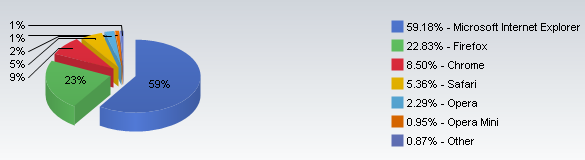
\includegraphics[height=3.5cm]{webbrowsers-share-2010-10}
% 
% \begin{flushright}
% Net Market Share Report, October 2010 \\
% {\small \url{http://www.netmarketshare.com/}}
% \end{flushright}
% \end{frame}

%%---------------------------------------------------------------------
% \subsection{References}
% 
% %%---------------------------------------------------------------
% 
% \begin{frame}
% \frametitle{References on linear models}
% 
% \begin{itemize}
%  \item \small [Faraway, 2005] Faraway, J. (2005) Linear models with R. CRC Press.
%  \item \small [Crawley, 2007] Crawley, M. J. The R book. Wiley.
%  \item \small [Kutner et al., 2004] Kutner, M., Nachtsheim, C., Neter, J. and Li, W. (2004).
% Applied Linear Statistical Models. McGraw-Hill.
% 
%  \end{itemize}
% \end{frame}
% 
% %%---------------------------------------------------------------
% 
% \begin{frame}
% \frametitle{Linear models with R}
% 
% \begin{itemize}
%  \item \small [Faraway, 2002] Faraway, J. Practical Regression and Anova Using R.
%  \url{http://cran.r-project.org/doc/contrib/Faraway-PRA.pdf}
% 
%  \item \small [Faraway, 2002] Faraway, J. Introduction to Probability and Statistics Using R.
%  \url{http://www.lulu.com/items/volume_68/8123000/8123594/3/print/IPSUR.pdf}
% 
%  \end{itemize}
% \end{frame}

%%---------------------------------------------------------------
